% id: 181-14
% book: 베이직쎈 대수 · 10 등비수열
% section: 실전 감각 UP
% figure: tikz:fig-181-14
% answer: 
% answer_source: 
% variant_level: 0 (원본 전사)
% 이 파일은 build.mjs 가 items.json 에서 만든다. 고칠 때는 items.json 을 고친다.
\smash{\raisebox{1.5mm}{\dmkichul{베이직쎈 대수 181쪽 14번 · 꼭 나와요}}}
\noindent\begin{minipage}[t]{0.58\linewidth}\vspace{0pt}\raggedright 한 변의 길이가 $6$인 정삼각형이 있다. 1회 시행에서 오른쪽 그림과 같이 각 변의 중점을 이어 정삼각형을 그린다. 2회 시행에서는 1회 시행에서 그린 작은 정삼각형에 같은 방법으로 정삼각형을 그린다. 이와 같은 시행을 계속할 때, 8회 시행에서 그린 정삼각형의 둘레의 길이를 구하시오.\end{minipage}\hfill\begin{minipage}[t]{0.4\linewidth}\vspace{0pt}\centering \resizebox{\ifdim\width>\linewidth\linewidth\else\width\fi}{!}{% 181-14(181쪽) — 한 변의 길이가 6인 정삼각형과 각 변의 중점을 이어 그린 정삼각형(1회 시행).
% 스캔 그림이라 화질이 낮아 TikZ 로 다시 그렸다. 원문에 있는 6 만 적고 8회 시행의 둘레(답)는 적지 않는다.
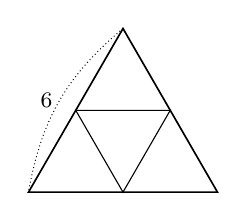
\begin{tikzpicture}[scale=0.4, line width=0.6pt]
  \coordinate (B) at (0,0);
  \coordinate (C) at (6,0);
  \coordinate (A) at (3,5.196);
  \coordinate (M) at (1.5,2.598);
  \coordinate (N) at (4.5,2.598);
  \coordinate (L) at (3,0);
  \draw (A) -- (B) -- (C) -- cycle;
  \draw[line width=0.4pt] (M) -- (N) -- (L) -- cycle;
  \draw[densely dotted, line width=0.35pt] (A)
    to[bend right=20] node[midway, left=-1pt, font=\footnotesize] {$6$} (B);
\end{tikzpicture}
}\end{minipage}\par
